\begin{figure}[!h]
\caption{Routine pc use by job type}
\subfloat[Below GCSE C]{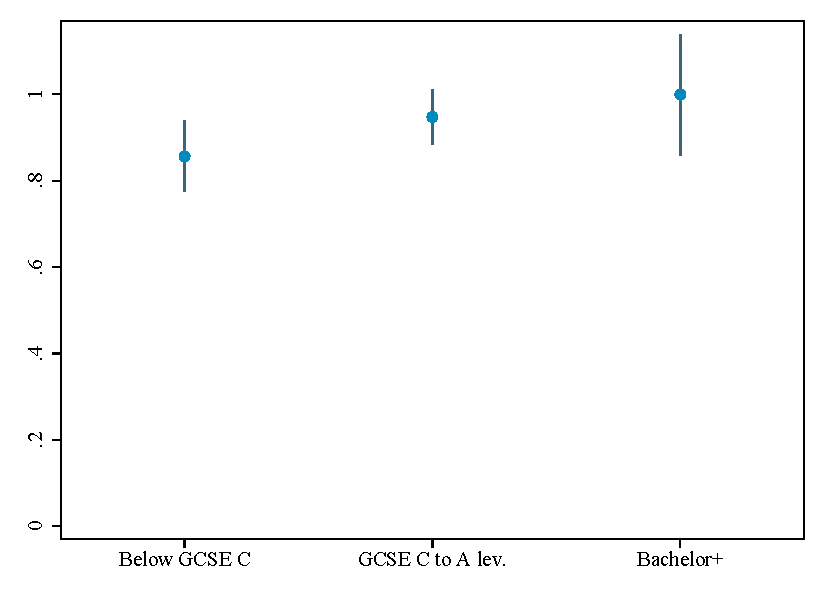
\includegraphics[width=.5\textwidth]{../output/routinepcuse1}} \subfloat[GCSE C-A levels]{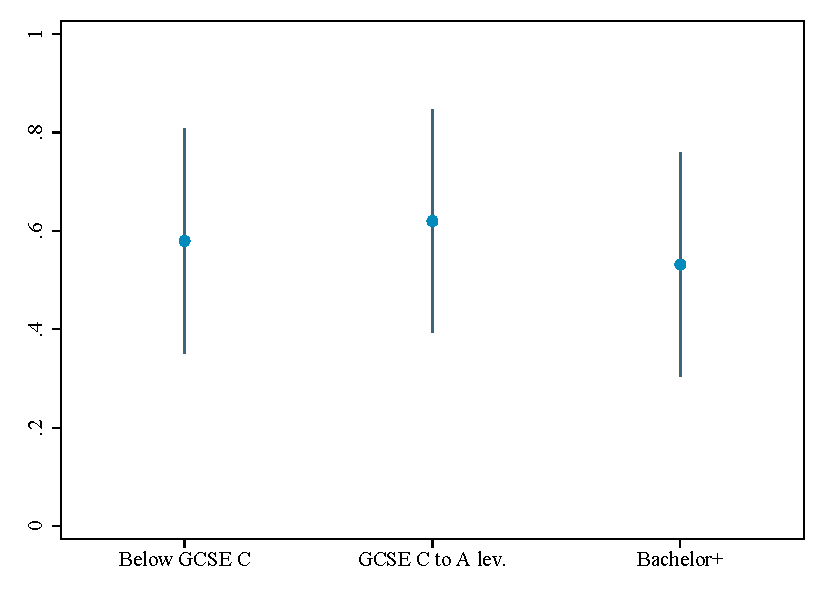
\includegraphics[width=.5\textwidth]{../output/routinepcuse2}} \\ \subfloat[Bachelor+]{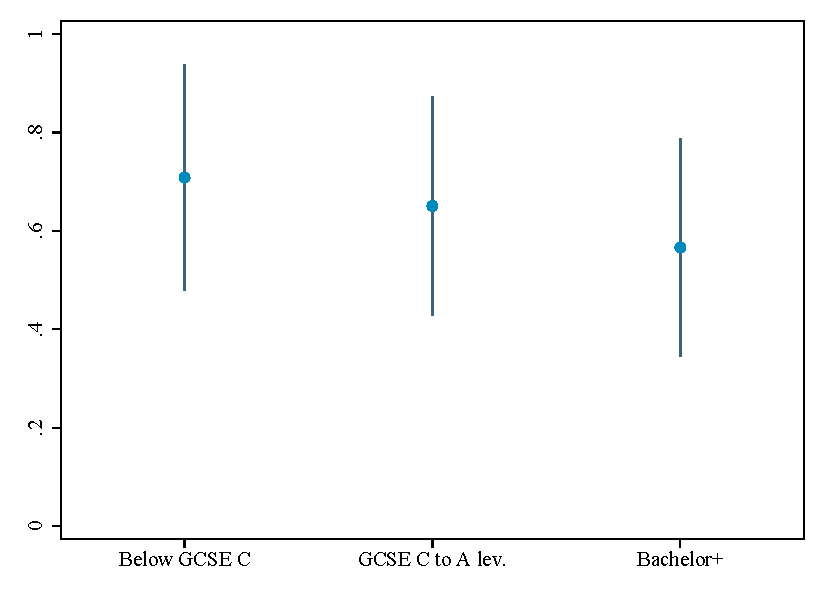
\includegraphics[width=.5\textwidth]{../output/routinepcuse3}} \subfloat[Below GCSE C/GCSE C-A levels]{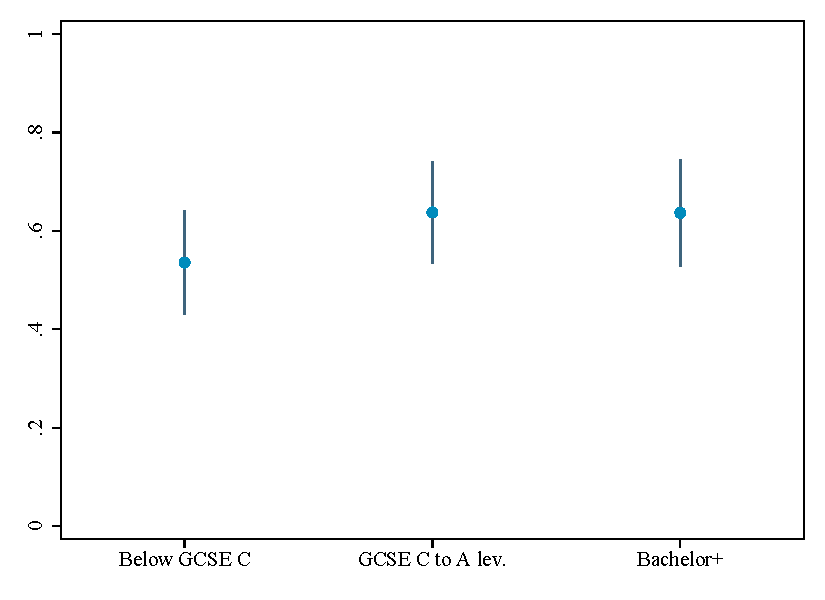
\includegraphics[width=.5\textwidth]{../output/routinepcuse12}} \\ \subfloat[GCSE C-A levels/Bachelor+]{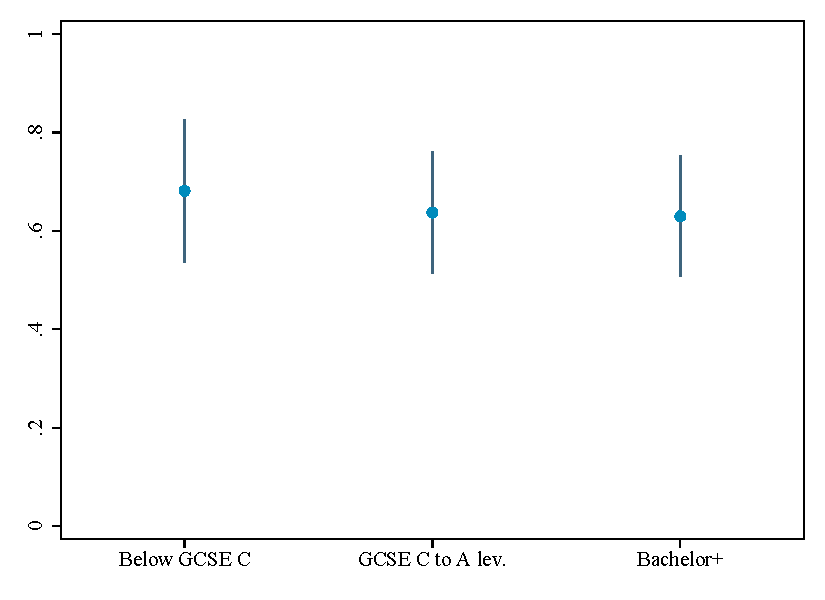
\includegraphics[width=.5\textwidth]{../output/routinepcuse23}} 
\par \begin{minipage}[h]{\textwidth}{\scriptsize\textbf{Note:} graphs show regression coefficients. Regressions include occupation and year fixed effects. CI based on robust standard errors. I assign a 0 to individuals who do not use a computer. I define routine use as declaring that one's pc use complexity is straightforward or moderate Figure generated on 12 Jun 2020 at 15:40:38. Figure generated using the dofile 3\_sesAnalysis/pcUseTables.do.}\end{minipage}
\end{figure}
